\documentclass[a4paper,11pt,twocolumn]{article}
\usepackage{graphicx,epsfig}
\usepackage{natbib}         % bibliography package
\usepackage{hyperref} 
\usepackage{times}
\usepackage[leftcaption]{sidecap}
\usepackage{fancyhdr}
\usepackage{subfigure}      % figures can have sub chunks
\usepackage{geometry}       % this maxes page usage, making the below unnecessary
\usepackage[cc]{titlepic}   % allows a pic to be included in the title page
\usepackage[toc,page]{appendix} % allows for an appendix section
\usepackage[normalem]{ulem} % for table
\useunder{\uline}{\ul}{}    % for table
\usepackage{listings}       % code listings
\usepackage{color}          % code listings colours
\usepackage{gensymb}        % degree sign
\usepackage{amsmath}        % matrices

\textwidth = 6.75in
\oddsidemargin = -0.25in
\textheight = 10in
\topmargin = -0.5in

% definitions for fancyhdr package
\pagestyle{fancy}
\lhead{{\it A. Jaamour, A. Lissak}}
\chead{Computer Vision}
\rhead{CM30080 Coursework}
\lfoot{}
\cfoot{\thepage}
\rfoot{}

\definecolor{codegreen}{rgb}{0,0.6,0}
\definecolor{codegray}{rgb}{0.5,0.5,0.5}
\definecolor{codepurple}{rgb}{0.58,0,0.82}
\definecolor{backcolour}{rgb}{0.95,0.95,0.92}
 
% style for code listings
\lstdefinestyle{mystyle}{
    backgroundcolor=\color{backcolour},   
    commentstyle=\color{codegreen},
    keywordstyle=\color{magenta},
    numberstyle=\tiny\color{codegray},
    stringstyle=\color{codepurple},
    basicstyle=\footnotesize,
    breakatwhitespace=false,         
    breaklines=true,                 
    captionpos=b,                    
    keepspaces=true,                 
    numbers=left,                    
    numbersep=5pt,                  
    showspaces=false,                
    showstringspaces=false,
    showtabs=false,                  
    tabsize=2
}
\lstset{style=mystyle}

\newcommand{\goodgap}{
 \hspace{\subfigtopskip}
 \hspace{\subfigbottomskip}
}

\title{Filtering, Object Recognition and Features}
\author{Adam Jaamour, Andrea Lissak}

\renewcommand{\familydefault}{lmss}
%beautiful table
\usepackage[table]{xcolor}
\usepackage{longtable}
\usepackage{tabularx}
%\setlist{nolistsep}
\definecolor{orange}{HTML}{cd8641}
\definecolor{yellow}{HTML}{f0f4b2}
\definecolor{bordeaux}{HTML}{641113}

%%%%%%%%%%%%%%%%%%%%%%%%%%%%%%%%%%%%%%%%%%%%%%%%%%%%%%%%%%%%%%%%%%%%%%%%
%%%%%%%%%%%%%%%%%%%%%%%%%%%%%%%%%%%%%%%%%%%%%%%%%%%%%%%%%%%%%%%%%%%%%%%%
%%%%%%%%%%%%%%%%%%%%%%%%%%%%%%%%%%%%%%%%%%%%%%%%%%%%%%%%%%%%%%%%%%%%%%%%

\begin{document}
\maketitle
\clearpage

\section{Choice of Language: Python}

For this project, the programming language of choice was Python. It was chosen over MATLAB due to the availability of functions similar to MATLAB's functions through libraries, and due to the syntax and flexibility of the language. With libraries such as OpenCV for image manipulations, Numpy and SciPy for more advanced mathematical functions including array manipulations, and MatPlotLib for plotting data, Python has all the tools for the task at hand.

%%%%%%%%%%%%%%%%%%%%%%%%%%%%%%%%%%%%%%%%%%%%%%%%%%%%%%%%%%%%%%%%%%%%%%%%
%%%%%%%%%%%%%%%%%%%%%%%%%%%%%%%%%%%%%%%%%%%%%%%%%%%%%%%%%%%%%%%%%%%%%%%%
%%%%%%%%%%%%%%%%%%%%%%%%%%%%%%%%%%%%%%%%%%%%%%%%%%%%%%%%%%%%%%%%%%%%%%%%

\section{Task 1: Image Convolution}

For the image convolution task, a function to perform convolution on a grey image was written. This function takes an image to operate on and a kernel to apply on the image. In order to preserve image size, extra padding is added on the edges of the original image. The function can be found in Listing \ref{lst:conv-function}.\\

Multiple filters are used to test the convolution function, including a Gaussian kernel, a sharpen kernel, a horizontal edge detector (Sobel filter) and an identity matrix. To confirm that the results are correct, the resulting filtered image compared to a library function. SciPy's ``\textit{convolve}'' function was used to carry out this task as it is the equivalent of MATLAB's ``\textit{conv2}'' function. The comparison is done by subtracting  the function's result from the library's result and checking that all the values are equal to 0. See Listing \ref{lst:conv-test} for the filters used and the test.

%%%%%%%%%%%%%%%%%%%%%%%%%%%%%%%%%%%%%%%%%%%%%%%%%%%%%%%%%%%%%%%%%%%%%%%%
%%%%%%%%%%%%%%%%%%%%%%%%%%%%%%%%%%%%%%%%%%%%%%%%%%%%%%%%%%%%%%%%%%%%%%%%
%%%%%%%%%%%%%%%%%%%%%%%%%%%%%%%%%%%%%%%%%%%%%%%%%%%%%%%%%%%%%%%%%%%%%%%%

\section{Task 2: Intensity-Based Template Matching}

\subsection{Pre-Processing}

Multiple steps are followed to pre-process the training dataset. Firs, The background is set to 0 for each image in the training dataset. This is done by looking for white pixels (value 255) and replacing them with black pixels (value 0), as depicted in Listing \ref{lst:preprocessing} line 3. Next, each rotated and scaled template in the pyramid is then normalised using OpenCV's ``\textit{normalize}'' function, which can be found in Listing \ref{lst:preprocessing} line 10. Finally, images are processed in RGB (3 channels) rather than being converting to grey scale (1 channel), therefore avoiding the loss of information and accuracy.

\subsection{Gaussian Pyramid Generation}

A Gaussian Pyramid is generated for each image in the training dataset. The scaling and rotation values for the pyramids were chosen by manually inspecting the training images to find out what angles the images were rotated to and by how much the images were scaled down. Therefore, scales of 50\%, 25\%, 12.5\% and 6.25\% were chosen, along with rotations ranging from 0\degree to 330\degree with steps of 30\degree for each scale. A brief overview of the training function used to generate the templates can be found in Listing \ref{lst:gaussian-pyramid}.\\

The rotation of the templates was achieved through SciPy's ``\textit{rotate}'' function (Listing \ref{lst:gaussian-pyramid}, line 22), while the scaling down was done manually with a custom subsampling function that recursively scales the image down by half by subsampling one pixel every two pixels (see Listing \ref{lst:subsample}). The subsampling blurring uses a Gaussian Filter with a size of 5x5 and a standard deviation $\sigma=15$.\\

Each template is saved in separate binary ``\textit{.dat}'' files for quicker I/O operations using Python's ``\textit{pickle}'' library for object serialisation conversion in byte streams (see Listing \ref{lst:gaussian-pyramid}, line 26).

\subsection{Output}

\subsubsection{Testing}

For the testing phase, each template previously stored in binary files is loaded in memory and is slid over one of the images from the testing dataset. All the templates for a single class are used to calculate the correlation score using Equation \ref{eq:corr}. The template with the highest score for a class is kept as the best match for that class, meaning there are 50 potential matching templates. Each template is then filtered based on its correlation score: it is kept if it is higher than a threshold, set at 0.5. This threshold is set empirically by testing different values until one that gave the most matches is found. \\

\begin{equation}
\label{eq:corr}
    cor(x,y) = \sum_{i,j} T(i,j) I(i+x, j+y)
\end{equation}

\subsubsection{Box Drawing}

The final step in producing the output is to draw a box around the detected objects that passed the threshold. The scaling and the rotation of the selected templates are used to draw the rectangle at the correct scale and at the correct rotation (see Listing \ref{lst:box-drawing}). The class name is drawn along with the box rather than class number to improve the output's clarity.\\

A rotated rectangle needs 4 pairs of coordinates to be drawn. Obtaining one pair will make it trivial to find the others. So, the real objective is to find the x and y shift from the one of the hypothetical straight square. Let us denote the x shift by $\Delta x$. Starting from a system of equation defining that the height/width of the original image is $h = \Delta x + \Delta y$, that $\sin(\alpha)*n = \Delta y$ and that $n^2 = \Delta x^2 + \Delta y^2$ (where \textit{n} is the length of the newly rotated and scaled square). So, resulting from the above, we can find $\Delta x$ (as shown in Equation \ref{eq:a}), thus all the corners of the rotated square: ($\sin(\alpha) = k$)

\begin{equation}\label{eq:a}
    \Delta x=\frac{\sqrt{h^2k^2-h^2k^4}+hk^2-h}{2k^2-1}
\end{equation}

\subsection{Results Evaluation}

To evaluate the results of our intensity-based template matching algorithm, the number of true and false positives are counted for each test along with the runtime measured in seconds. The results are reported in Figure \ref{fig:template-matching-results}. The average number of True Positives is 3.65, whereas the average number of False Positives is 31.2. This betrays the fact that this kind of matching algorithm is inefficient.\\

Attempts to maximise True Positives and minimise False Positives included increasing the threshold, which caused the number of False Positive matches to decrease but had a ripple effect on True Positive matches that were filtered out as well. A case that was often observed was that many small templates often matched with large images with white backgrounds such as ``airport'' or ``bank'', meaning they could either not be matched with the correct object or were not filtered out by the threshold due to their high correlation score with the white background. The correlation method does not provide a difference that important enough to efficiently filter out False Positives without affecting the True Positives.\\

Other more successful improvements consist in fine-tuning the Gaussian filter. Using a Gaussian filter of size $5x5$ with $\sigma=15$ allows a minimal amount of artefacts to appear in the templates when scaling down images, thus increasing accuracy. Additionally, the templates are generated in RGB rather than grey scale. The improvement in accuracy was drastic as less templates matched with white backgrounds when using colours. With more time, an additional enhancement could have been implemented by drawing a box for only the best matching template around a single location with an object on the test image, which would limit the number of false positives around a single object.

\begin{figure}[!htbp]
\centering
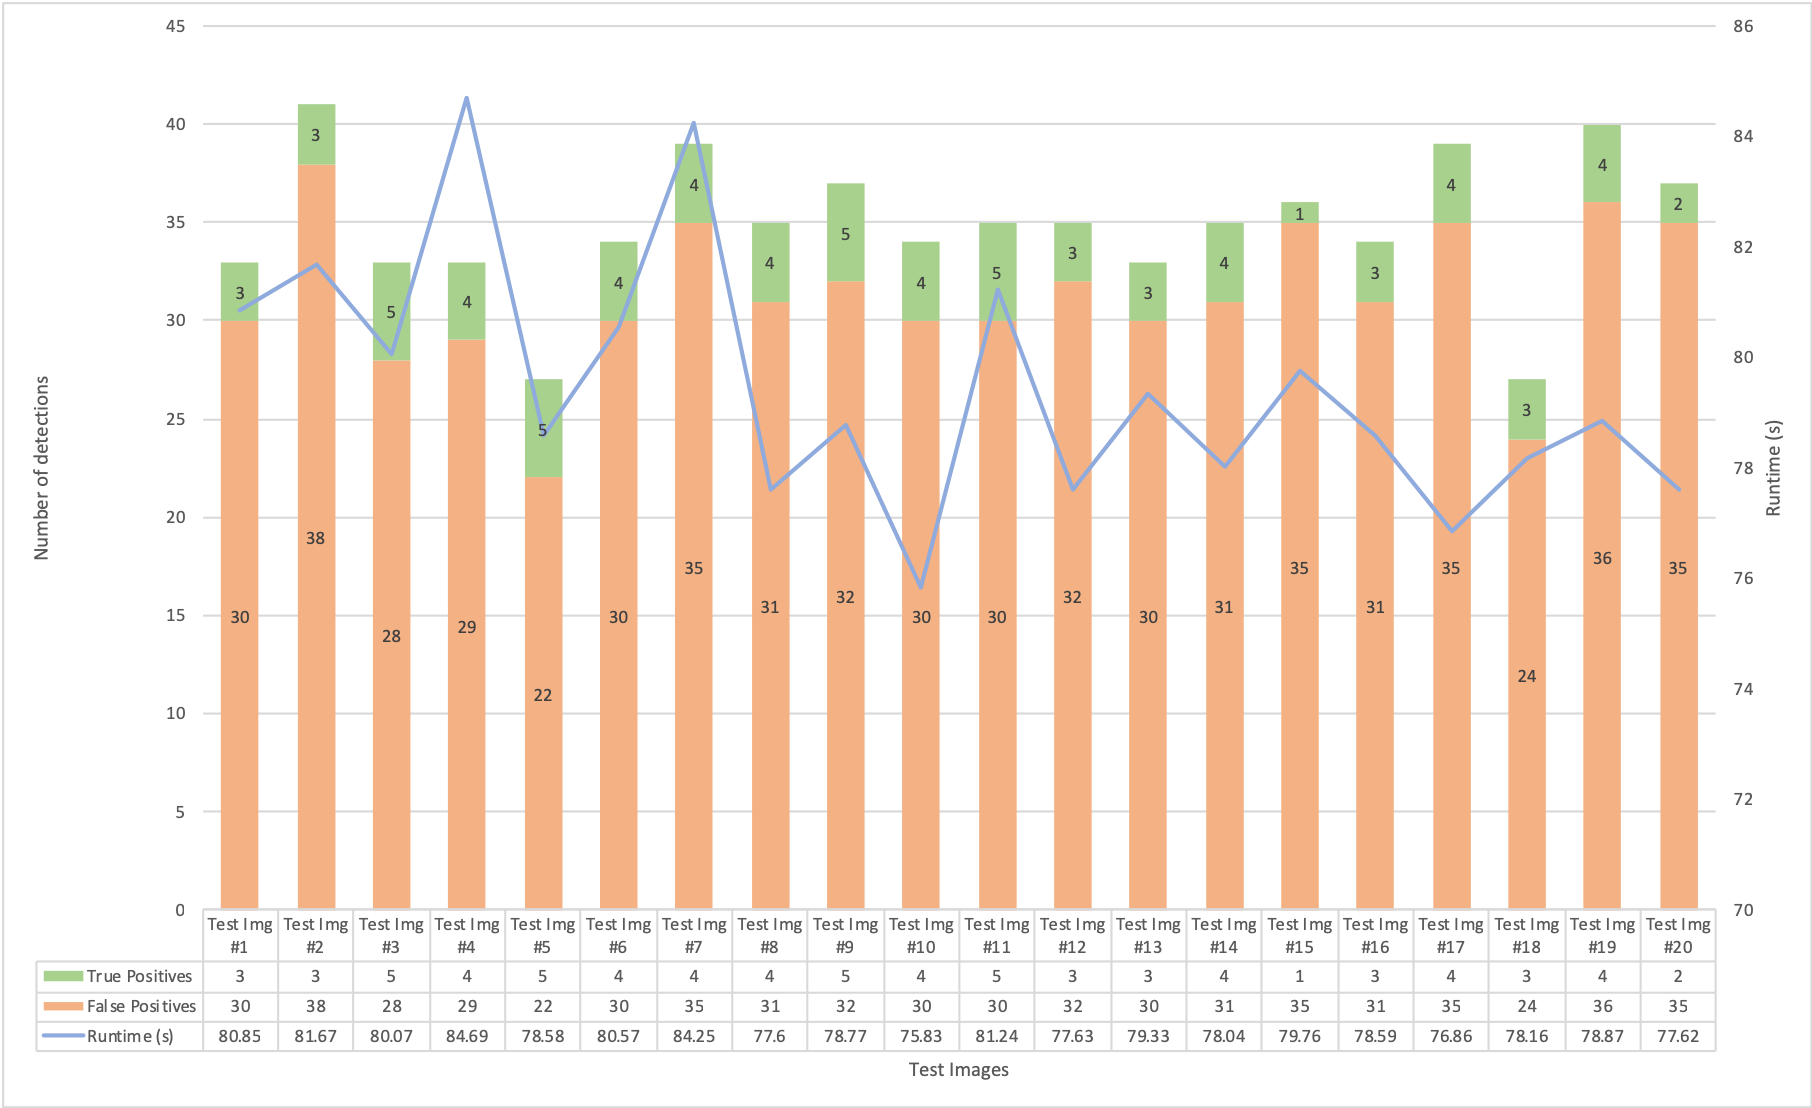
\includegraphics[scale=0.25]{figures/evaluation.png}
\caption{Results of Task 2 for each image in the testing dataset. In green, the number of true positive matches, in red the number of false positive matches, and in blue the runtime measured in seconds.}
\label{fig:template-matching-results} 
\end{figure}

The complexity of the training function that generates the Gaussian Pyramid is $O(p*r*n^2)$ per image per colour channel, where \textit{n} corresponds to the image size (e.g. \textit{n} would be 262144 for a 512 by 512 image, and not 512), \textit{p} to the number of scales and \textit{r} to the number of rotations. Therefore the problem size increases linearly for each image added to the training dataset. However, the scalability is extremely inefficient when it comes to the testing. Indeed, with our current choice of scales and rotations, each new image in the training set would add 48 additional templates to slide across the test image, which currently takes on average 79.45 seconds with 2400 templates to slide across the test image.

%%%%%%%%%%%%%%%%%%%%%%%%%%%%%%%%%%%%%%%%%%%%%%%%%%%%%%%%%%%%%%%%%%%%%%%%
%%%%%%%%%%%%%%%%%%%%%%%%%%%%%%%%%%%%%%%%%%%%%%%%%%%%%%%%%%%%%%%%%%%%%%%%
%%%%%%%%%%%%%%%%%%%%%%%%%%%%%%%%%%%%%%%%%%%%%%%%%%%%%%%%%%%%%%%%%%%%%%%%

\section{Task 3: SIFT Features}
Scale-invariant feature transform, as described by \citet{lowe2004distinctive}, can be interpreted as a pipeline. So, the following paragraphs will go through the results of an attempt of implementation of SIFT. (The choice of constants for the current implementation consisted in following \citet{lowe2004distinctive}'s recommendations). As a high-level indication, all that is explained below was carried out through three different samplings originating from the original image (three octaves).

\subsection{Key-point Filtering}
Key-points are points of interest of an image. Therefore, when looking for them, a threshold for low contrast can be used for early filtering less relevant key-points. Now that only high-change areas have been spotted, extrema can be found, i.e. sharper changes which refer to edges and corners in the original image. Applying a Laplacian filter is an appropriate solution for such task. However, in discrete domains it has been found that the \textit{Difference of Gaussians} (\textit{DoG}) is a relatively accurate approximation to enable interest point localisation \citep{lowe1999object}. Peaks and dips are spotted by comparing multiple differences of Gaussians together. So, \textit{DoG} ($\sigma_{2}$, $\sigma_{3}$) will be compared with the adjacent layers ($\sigma_{1}$, $\sigma_{2}$) and ($\sigma_{3}$, $\sigma_{4}$). More specifically, each analysed candidate will be compared with its 26 neighbouring candidates (8 within the same scale, 18 ranging between the above and below scales). Once all the minima and maxima are extracted, more keypoint can be filtered out by eliminating edges, which contain less information than corners. Because eigenvalues are discrete indicators, they can be used to discriminate these two cases. Consequently, a threshold to filter out edges can be applied. The code for this section can be found in Listing \ref{lst:sift-keypoints-filtering}. 

\subsection{Key-point Magnitude and Orientation}
At this point, the coordinates of the key-points have been selected. In order to diversify them further, given their neighbourhood, both their magnitude and their orientation can be calculated. This is achieved by looking at pixel differences, meaning that pixel intensities arranged in certain ways can output how sharp a feature is and what its rotation is. This is applied across the entire image as it is a useful foundation for the following step, which corresponds to assigning a noise-free orientation and magnitude for each of the key-points. To enforce this, each key-point's neighbourhood needs to be taken into account. The code for this section can be found in Listing  \ref{lst:magnitude-orientation}.\\

A Gaussian distribution centred around the key-point is used to give more importance to pixels that are close to the key-point than to further ones. This means that each time one of these neighbours is visited, one of 36 rotation buckets corresponding to its orientation (divided by a factor of ten, to be more easily computed in discrete form) is increased by the calculated weight. In the end, once the whole neighbourhood is visited, the algorithm looks at the bucket that is the most full. In \citet{lowe2004distinctive}'s implementation, buckets which are 80\% (or more) of the largest one are used to spawn new key-points with different rotations. However, in the current, this has not been implemented given the consequences being fairly negligible. The output is thus the key-point matrix, which includes $(x, y)$, $m(x, y)$ and $\theta(x, y)$.

\subsection{Box Representation}
The key-point matrix can be used to visualise the location, magnitude and orientation of interest points on the original images. In our implementation, this has been done by placing markers with the radius directly proportional to the key-point's scale and with segments matching the orientation, as demonstrated in Figure \ref{fig:sift-key-points} (see the function used to draw these in Listing \ref{lst:sift-draw-boxes}).

\begin{figure}[!htbp]
\centering
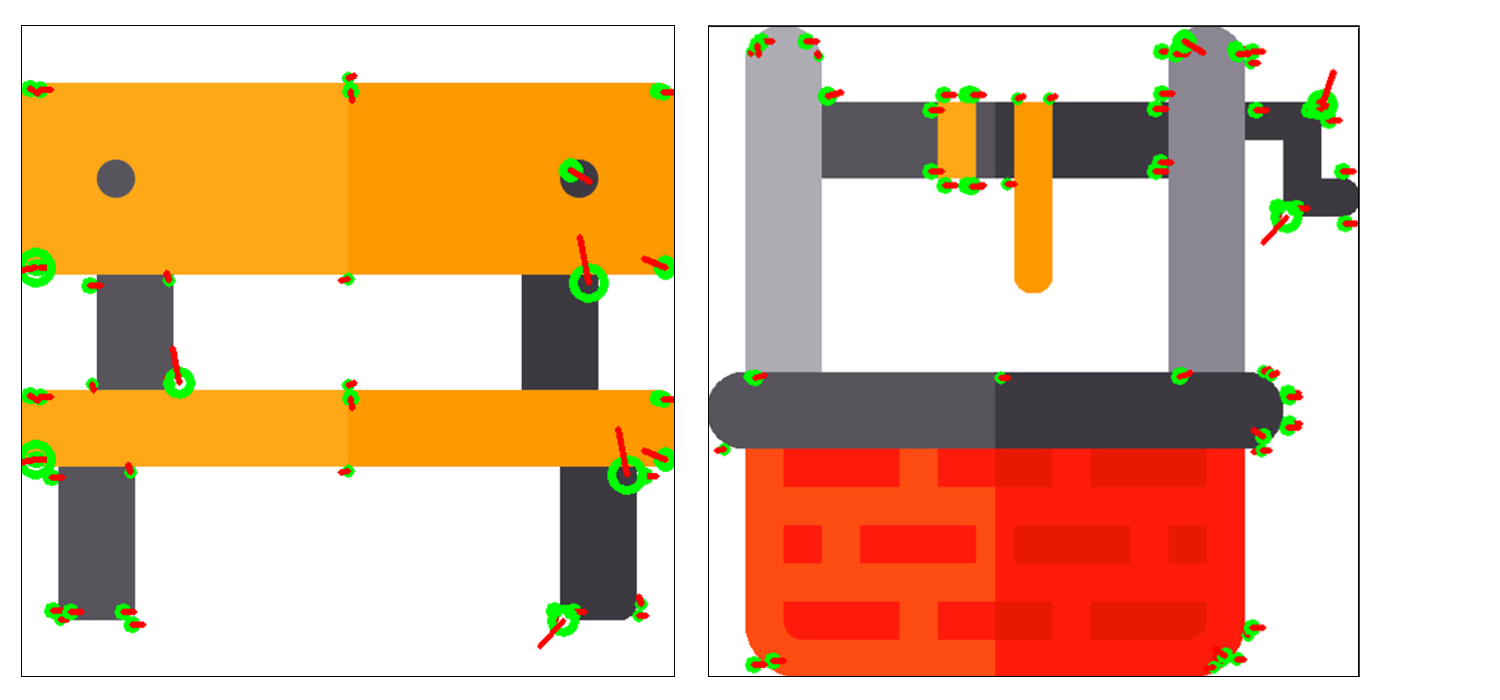
\includegraphics[scale=0.12]{figures/sift-key-points.png}
\caption{SIFT key points on 2 training images.}
\label{fig:sift-key-points} 
\end{figure}

\subsection{Descriptors}
Descriptors are used to keep track of the bucket-style histogram representation of neighbouring areas. \citet{lowe2004distinctive}'s measures have been used for this, which means that this program generates 16 histograms, each made up of 16 pixels. The number of buckets used to maximise performance is 8 \citep{lowe2004distinctive}. Therefore, a total of 16 histograms with 8 buckets each (128 values) are used to define the descriptor for each key-point. The code for this section can be found in Listing \ref{lst:descriptors}.

%%%%%%%%%%%%%%%%%%%%%%%%%%%%%%%%%%%%%%%%%%%%%%%%%%%%%%%%%%%%%%%%%%%%%%%%
%%%%%%%%%%%%%%%%%%%%%%%%%%%%%%%%%%%%%%%%%%%%%%%%%%%%%%%%%%%%%%%%%%%%%%%%
%%%%%%%%%%%%%%%%%%%%%%%%%%%%%%%%%%%%%%%%%%%%%%%%%%%%%%%%%%%%%%%%%%%%%%%%

\raggedright
\bibliographystyle{apalike}
\bibliography{bibliography}

\onecolumn
\clearpage

\begin{table}[h]
\resizebox{\textwidth}{!}{%
\begin{tabular}{|r|c|c|}
\hline
\textbf{Student Name}            & {\ul Adam Jaamour}                                                                                                                      & {\ul Andrea Lissak}                                                                                                             \\ \hline
\textbf{Student Username}        & \textit{aj645}                                                                                                                          & \textit{al746}                                                                                                                  \\ \hline
\textbf{Student ID}              & \textit{159327001}                                                                                                                      & \textit{159044728}                                                                                                              \\ \hline
\textbf{Contributions}           & \multicolumn{1}{l|}{\textit{\begin{tabular}[c]{@{}l@{}}- Convolution\\ - intensity-based template \\   matching training\end{tabular}}} & \multicolumn{1}{l|}{\textit{\begin{tabular}[c]{@{}l@{}}- SIFT\\ - intensity-based template \\   matching testing\end{tabular}}} \\ \hline
\textbf{Contribution Percentage} & \textit{50\%}                                                                                                                           & \textit{50\%}                                                                                                                   \\ \hline
\end{tabular}%
}
\end{table}

\clearpage
\begin{appendices}

\section{Convolution Function}
\lstinputlisting[label={lst:conv-function},language=Python]{code-listings/convolution/convolution.py}

\section{Convolution Filters Test}
\lstinputlisting[label={lst:conv-test},language=Python]{code-listings/convolution/convolution-testing.py}

\section{Intensity-Based Template Matching Pre-processing}
\lstinputlisting[label={lst:preprocessing},language=Python]{code-listings/template-matching/pre-processing.py}

\clearpage
\section{Intensity-Based Template Matching Gaussian Pyramid}
\lstinputlisting[label={lst:gaussian-pyramid},language=Python]{code-listings/template-matching/gaussian-pyramid.py}

\section{Intensity-Based Template Matching Subsampling Function}
\lstinputlisting[label={lst:subsample},language=Python]{code-listings/template-matching/subsample.py}

\clearpage
\section{Intensity-Based Template Matching Testing}
\lstinputlisting[label={lst:testing},language=Python]{code-listings/template-matching/testing.py}

\section{Intensity-Based Template Matching Box Scaling/Rotating}
\lstinputlisting[label={lst:box-drawing},language=Python]{code-listings/template-matching/find_box_corners.py}

\clearpage
\section{SIFT Key Points Filtering}
\lstinputlisting[label={lst:sift-keypoints-filtering},language=Python]{code-listings/sift/keypoint-filtering.py}

\section{SIFT Magnitude and Orientation}
\lstinputlisting[label={lst:magnitude-orientation},language=Python]{code-listings/sift/magnitude-orientation.py}

\section{SIFT Descriptors}
\lstinputlisting[label={lst:descriptors},language=Python]{code-listings/sift/descriptors.py}

\section{SIFT Box Drawing with Direction}
\lstinputlisting[label={lst:sift-draw-boxes},language=Python]{code-listings/sift/sift-draw-boxes.py}

\end{appendices}
\end{document}